\documentclass{article}[18pt]
\usepackage{../../../../format}
\lhead{Networks and Systems - Networks}


\begin{document}
\begin{center}
\underline{\huge Transport Layer (part 1)}
\end{center}
\section{Transport-layer services}
\subsection{Transport services and protocols}
\begin{itemize}
	\item Provide logical communication between app processes running on different hosts
	\item Transport protocols run in end systems
	\begin{itemize}
		\item Send side: breaks up app messages into segments, passes to network layer
		\item Receive side: reassembles segments into messages, passes to app layer
	\end{itemize}
	\item More than one transport protocol available to apps:
	\begin{itemize}
		\item Internet: TCP and UDP
	\end{itemize}
\end{itemize}
\subsection{Transport vs network layer}
\begin{defin}[Network layer]
Logical communication between hosts
\end{defin}
\begin{defin}[Transport layer]
Logical communication between processes. Relies on and enhances network layer services
\end{defin}
\subsection{Internet transport-layer protocols}
TCP (Transmission Control Protocol):
\begin{itemize}
	\item Reliable, in-order delivery
	\item Congestion control
	\item Flow control, ack., timer
	\item Connection setup
\end{itemize}
UDP(User Datagram Protocol):
\begin{itemize}
	\item Unreliable, unordered delivery
	\item No-frills extension of "best-effort" IP
	\item Services not available
	\item Delay guarantees
\end{itemize}
TCP and UDP extend IP delivery service between hosts to delivery service between processes $\rightarrow$ transport layer multiplexing and demultiplexing
\section{Multiplexing and demultiplexing}
\begin{center}
	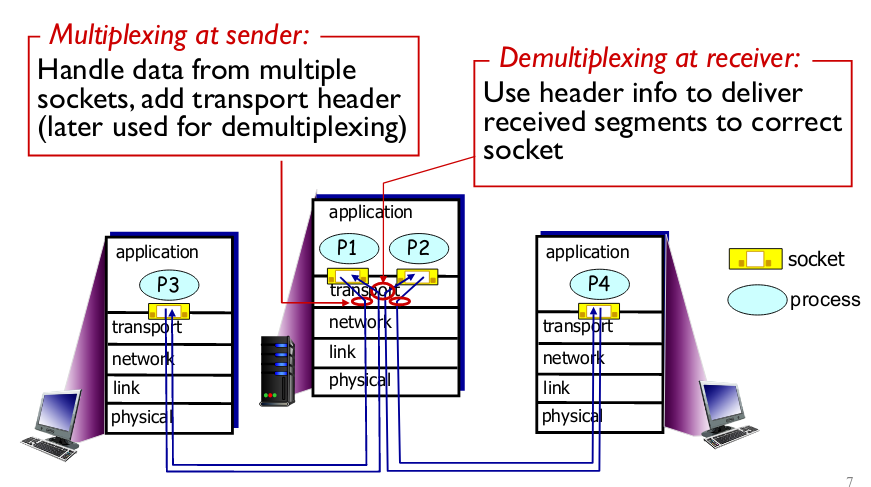
\includegraphics[scale=0.7]{multiplexing}
\end{center}
\begin{itemize}
	\item Host receives IP datagrams
	\item Each datagram has source IP address, destination IP address
	\item Each datagram carries one transport-layer segment
	\item Each segment has source, destination port number
	\item Host uses IP addresses and port numbers to direct segment to appropriate socket
	\item Each socket has a unique identifier
\end{itemize}
\begin{center}
	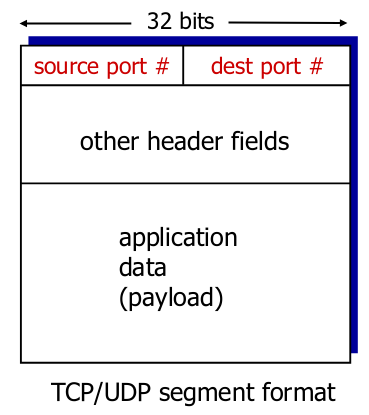
\includegraphics[scale=0.7]{segment}
\end{center}
\subsection{Connectionless multiplexing and demultiplexing}
\begin{itemize}
	\item All sockets have host-local port \#
	\item Assigned automatically, or via \texttt{bind()}
	\item \texttt{serverSocket,bind((ip, port))}
	\item When host receives UDP segment:
	\begin{itemize}
		\item Checks destination port \# in segment
		\item Directs UDP segment to socket with that port \#
	\end{itemize}
\end{itemize}
If two UDP segments have different source IP addresses and/or source port numbers but same dest IP and port \#, they will be directed to same process via same process via same socket as dest
\begin{center}
	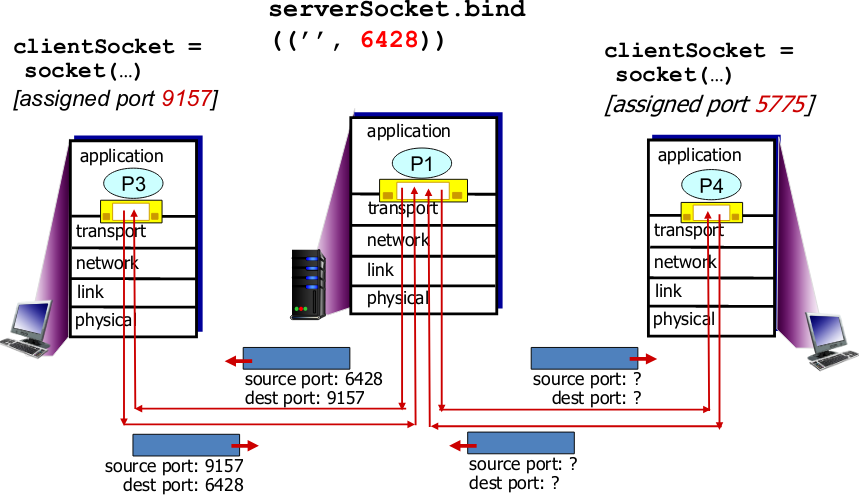
\includegraphics[scale=0.7]{demultiplexing}
\end{center}
\subsection{Connection-oriented multiplexing and demultiplexing}
TCP socket identified by 4-tuple
\begin{itemize}
	\item Source IP address
	\item Source port number
	\item Destination IP address
	\item Destination port number
\end{itemize}
Demix: receiver used all four values to direct segment to appropriate socket\\
Server host may support many simultaneous TCP sockets:
\begin{itemize}
	\item each socket identified by its own 4-tuple
	\item Two arriving TCP segments with different source IP/ \#Port will be directed to two different sockets
\end{itemize}
\begin{center}
	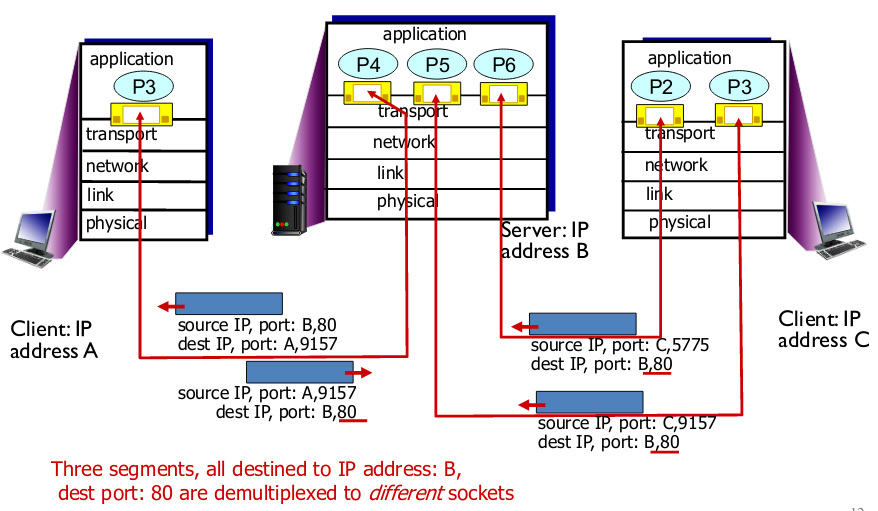
\includegraphics[scale=0.7]{connection}
\end{center}
\section{Connectionless transport: UDP}
\begin{itemize}
	\item "No frills", "bare bones" internet transport protocol
	\item "Best effort" service, UDP segments may be
	\begin{itemize}
		\item Lost
		\item Delivered out-of-order to app
	\end{itemize}
	\item Connectionless:
	\begin{itemize}
		\item No handshaking between sender/receiver
		\item Each UDP segment handled independently of others
	\end{itemize}
	\item UDP use:
	\begin{itemize}
		\item Streaming multimedia apps (loss tolerant, rate sensitive)
	\end{itemize}
	\item Reliable transfer over UDP
	\begin{itemize}
		\item Add reliability at application layer
		\item Application-specific error recovery
	\end{itemize}
\end{itemize}
\subsection{Segment Header}
\begin{center}
	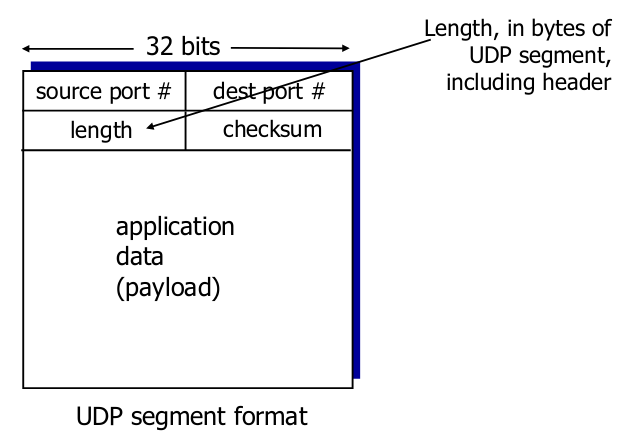
\includegraphics[scale=0.7]{udp}
\end{center}
\section{Principles of reliable data transfer}
\begin{center}
	\includegraphics[scale=0.7]{"reliable data transfer"}
\end{center}
\begin{center}
	\includegraphics[scale=0.7]{"reliable data transfer1"}
\end{center}

\end{document}